\section{Introduction}

% Introduce the discrete energy minimization problem
Discrete energy minimization, also known as min-sum labeling~\cite{Werner-PAMI07} or weighted constraint satisfaction (WCSP)\footnote{WCSP is a more general problem, considering a bounded plus operation.
% ::: what does bounded plus mean?
% ** in energy minimization, the all potentials are added together, there can be different operations to combine these potentials to form an objective in WCSP
It is itself a special case of valued CSP, where the objective takes values in a more general valuation set.}~\cite{jeavons2014complexity}, is a popular model for many problems in computer vision, machine learning, bioinformatics, and natural language processing. In particular, the problem arises in maximum a posteriori (MAP) inference for Markov (conditional) random fields (MRFs/CRFs)~\cite{Lauritzen96}.  In the most frequently used pairwise case, the {\em discrete energy minimization problem} (simply ``energy minimization'' hereafter) is defined as
\begin{align} \label{eq:1}
\min_{x\in\mathcal{L}^\V} \sum_{u\in\mathcal{V}} f_u(x_u) + \sum_{(u,v)\in\mathcal{E}} f_{uv}(x_u,x_v),
\end{align}
where $x_u$ is the label for node $u$ in a graph $\mathcal{G}=(\mathcal{V}, \mathcal{E})$. When the variables $x_u$ are binary (Boolean): $\L = \Bool = \{0,1\}$, the problem can be written as a quadratic polynomial in $x$~\cite{BorosHammer02} and is known as quadratic pseudo-Boolean optimization (QPBO)~\cite{BorosHammer02}. 
% The well-known quadratic pseudo-Boolean optimization (QPBO) is obtained when the variables $x_u$ are binary (Boolean): $\L = \Bool = \{0,1\}$, as the problem can be written as a quadratic polynomial in $x$~\cite{BorosHammer01}. 

% How does discrete energy minimization relate to Computer Vision?
In computer vision practice, energy minimization has found its place in semantic segmentation~\cite{ren2012rgb}, pose estimation \cite{yang2011articulated}, scene understanding  \cite{schwing2012efficient}, depth estimation \cite{liu2010single}, optical flow estimation \cite{xu2012motion}, image in-painting \cite{shekhovtsov-2012-curvature}, and image denoising \cite{barbu2009learning}.
For example, tree-structured models have been used to estimate pictorial structures such as body skeletons or facial landmarks~\cite{yang2011articulated}, multi-label Potts models have been used to enforce a smoothing prior for semantic segmentation~\cite{ren2012rgb}, and general pairwise models have been used for optimal flow estimation~\cite{xu2012motion}.
However, it may not be apparent that the energy minimization formulations used to model these vision problems have greatly varied degrees of tractability or {\em computational complexity}. For the three examples above, the first allows efficient exact inference, the second admits a constant factor approximation, and the third has no quality guarantee on the approximation of the optimum. 

% http://cvlab-dresden.de/wp-content/uploads/2016/01/inference.pdf
% http://cvlab-dresden.de/wp-content/uploads/2015/12/learning.pdf
%

% Brief review of complexity theory
The study of complexity of energy minimization is a broad field. Energy minimization problems are often intractable in practice except for special cases.  While many researchers analyze the time complexity of their algorithms (e.g., using big O notation), it is beneficial to delve deeper to address the difficulty of the underlying problem.  The two most commonly known complexity classes are P (polynomial time) and NP (nondeterministic polynomial time: all problems whose solutions can be verified in polynomial time). However, these two complexity classes are only defined for {\em decision} problems. The analogous complexity classes for {\em optimization} problems are PO (P optimization) and NPO (NP optimization: all optimization problems whose solution feasibility can be verified in polynomial time). Optimization problems form a superset of decision problems, since any decision problem can be cast as an optimization over the set $\{$yes, no$\}$, \ie, P $\subseteq$ PO and NP $\subseteq$ NPO. The NP-hardness of an optimization problem means it is at least as hard as (under Turing reduction) the hardest decision problem in the class NP. If a problem is NP-hard, then it is not in PO assuming P $\neq$ NP. 

% Approximations and the APX and exp-APX classes
Although optimal solutions for problems in NPO, but not in PO, are intractable, it is sometimes possible to guarantee that a good solution (i.e., one that is worse than the optimal by no more than a given factor) can be found in polynomial time.  These problems can therefore be further classified into class APX (constant factor approximation) and class exp-APX (inapproximable) with increasing complexity (Figure~\ref{fig:hardnessaxis}).  We can arrange energy minimization problems on this more detailed complexity scale, originally established in \cite{ausiello1999complexity}, to provide vision researchers a new viewpoint for complexity classification with a focus on NP-hard optimization problems.


% Overview of our new results
% Summary of contributions
In this paper, we make three core contributions, as explained in the next three paragraphs. First, we prove the inapproximability result of QPBO and general energy minimization. Second, we show that the same inapproximability result holds when restricting to planar graphs with three or more labels.
%In the proof, we propose a novel micro-graph structure-based reduction that can be used for algorithmic design as well. 
Finally, we present a unified framework and an overview of vision-related special cases where the energy minimization problem can be solved in polynomial time or approximated with a constant, logarithmic, or polynomial factor. 


\begin{figure}
\begin{center}
   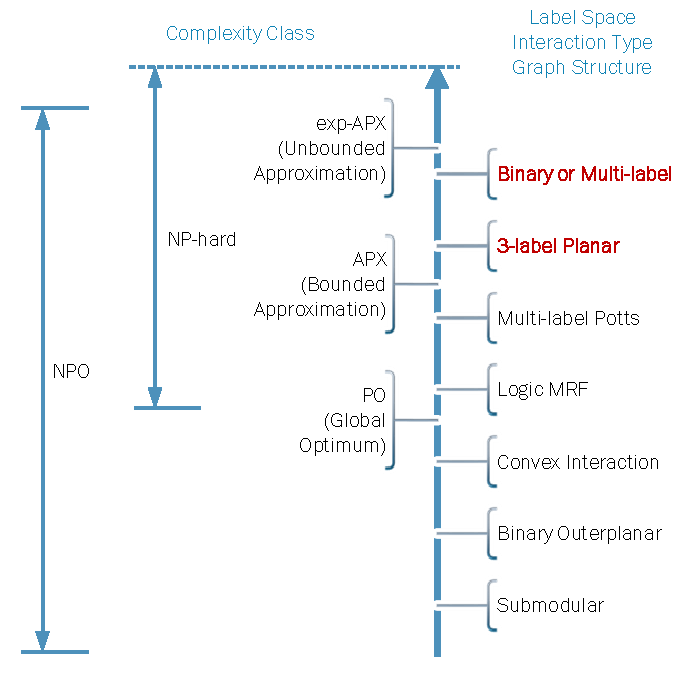
\includegraphics[width=0.6\linewidth]{figure/HardnessAxis.pdf}
\end{center}
    \caption{Discrete energy minimization problems aligned on a complexity axis. Red, boldface indicates new results proven in this paper. Note that problems are not ranked within a complexity class. Some problems discussed in this paper are removed for the simplicity of the figure.}
    % ** within a complexity class is not technically correct
\label{fig:hardnessaxis}
\end{figure}

% First contribution  QPBO and general case proof 
\textbf{Binary and multi-label case}  (Section~\ref{sec:gencase}). It is known that QPBO (2-label case) and the general energy minimization problem (multi-label case) are NP-hard~\cite{BorosHammer02}. They generalize such classical NP-hard optimization problems on graphs as vertex packing (maximum independent set) and the minimum and maximum cut problems~\cite{Karp-72}.
In this paper, we show a much stronger conclusion. \emph{We prove that QPBO as well as general energy minimization are complete (being the hardest problems) in the class exp-APX.} This implies that a polynomial time method cannot have a guarantee to find an approximation within a constant or even polynomially large factor of the optimum (assuming P$\neq$NP).
%This implies that there can be no method in polynomial time to find an approximation within a constant or even polynomial factor of the optimum. %, {\red and in fact, the only possible factor in polynomial time is exponential in the input size}. % please delete if unsure
In practice, this means that a solution may be essentially arbitrarily bad.
Furthermore, all optimization problems in which merely finding any feasible solution, disregarding the objective, is tractable (\eg, traveling salesman problem) are in exp-APX (see \Section{sec:prelim}) and thus QPBO, being exp-APX-complete, is amongst the hardest of such problems.
%In fact, any optimization problem, in which merely finding a feasible solution is tractable can be reduced to QPBO while preserving approximation ratio. It means that QPBO is as 


% 3 or more label planar graph contribution
\textbf{Planar three or more label case}  (Section~\ref{sec:plcase}). Planar graphs form the underlying graph structure for many computer vision and image processing tasks. It is known that efficient exact algorithms exist for some special cases of planar 2-label energy minimization, such as outerplanar~\cite{Schraudolph-10}.  In this paper, we show that for the case of three or more labels, planar energy minimization is exp-APX-complete, which means these problems are as hard as general energy minimization. The complexity of planar 2-label case remains an open question.

\textbf{Subclass problems}  (Section~\ref{sec:specialcases}). Special cases for some energy minimization algorithms relevant to computer vision are known to be tractable. However, detailed complexity analysis of these algorithms is patchy and spread across numerous papers.  In Section~\ref{sec:specialcases}, we classify the complexity of these subclass problems and illustrate some of their connections.  Such an analysis can help computer vision researchers become acquainted with existing complexity results relevant to energy minimization and can aid in selecting an appropriate model for an application or in designing new algorithms.





